





\begin{code}[hide]%
\>[0]\AgdaKeyword{open}\AgdaSpace{}%
\AgdaKeyword{import}\AgdaSpace{}%
\AgdaModule{Data.Nat}\<%
\\
\>[0]\AgdaKeyword{open}\AgdaSpace{}%
\AgdaKeyword{import}\AgdaSpace{}%
\AgdaModule{Data.Fin}\AgdaSpace{}%
\AgdaKeyword{using}\AgdaSpace{}%
\AgdaSymbol{(}\AgdaDatatype{Fin}\AgdaSymbol{;}\AgdaSpace{}%
\AgdaInductiveConstructor{zero}\AgdaSymbol{;}\AgdaSpace{}%
\AgdaInductiveConstructor{suc}\AgdaSymbol{)}\<%
\\
\>[0]\AgdaKeyword{open}\AgdaSpace{}%
\AgdaKeyword{import}\AgdaSpace{}%
\AgdaModule{Data.Product}\AgdaSpace{}%
\AgdaSymbol{as}\AgdaSpace{}%
\AgdaModule{Prod}\AgdaSpace{}%
\AgdaKeyword{hiding}\AgdaSpace{}%
\AgdaSymbol{(}\AgdaFunction{map}\AgdaSymbol{)}\<%
\\
\>[0]\AgdaKeyword{open}\AgdaSpace{}%
\AgdaKeyword{import}\AgdaSpace{}%
\AgdaModule{Relation.Binary.PropositionalEquality}\AgdaSpace{}%
\AgdaKeyword{hiding}\AgdaSpace{}%
\AgdaSymbol{(}\AgdaOperator{\AgdaInductiveConstructor{[\AgdaUnderscore{}]}}\AgdaSymbol{)}\<%
\\
\>[0]\AgdaKeyword{open}\AgdaSpace{}%
\AgdaKeyword{import}\AgdaSpace{}%
\AgdaModule{Relation.Binary}\<%
\\
\>[0]\AgdaKeyword{open}\AgdaSpace{}%
\AgdaKeyword{import}\AgdaSpace{}%
\AgdaModule{Function}\<%
\\
%
\\[\AgdaEmptyExtraSkip]%
\>[0]\AgdaKeyword{module}\AgdaSpace{}%
\AgdaModule{array}\AgdaSpace{}%
\AgdaKeyword{where}\<%
\\
%
\\[\AgdaEmptyExtraSkip]%
\>[0]\AgdaComment{--\ Transitivity\ of\ equality,\ written\ infix\ for\ proof\ chains.}\<%
\\
\>[0]\AgdaKeyword{infixl}\AgdaSpace{}%
\AgdaNumber{2}\AgdaSpace{}%
\AgdaOperator{\AgdaFunction{\AgdaUnderscore{}⊡\AgdaUnderscore{}}}\<%
\\
\>[0]\AgdaOperator{\AgdaFunction{\AgdaUnderscore{}⊡\AgdaUnderscore{}}}\AgdaSpace{}%
\AgdaSymbol{:}\AgdaSpace{}%
\AgdaSymbol{∀}\AgdaSpace{}%
\AgdaSymbol{\{}\AgdaBound{A}\AgdaSpace{}%
\AgdaSymbol{:}\AgdaSpace{}%
\AgdaPrimitive{Set}\AgdaSymbol{\}}\AgdaSpace{}%
\AgdaSymbol{\{}\AgdaBound{x}\AgdaSpace{}%
\AgdaBound{y}\AgdaSpace{}%
\AgdaBound{z}\AgdaSpace{}%
\AgdaSymbol{:}\AgdaSpace{}%
\AgdaBound{A}\AgdaSymbol{\}}\AgdaSpace{}%
\AgdaSymbol{→}\AgdaSpace{}%
\AgdaBound{x}\AgdaSpace{}%
\AgdaOperator{\AgdaDatatype{≡}}\AgdaSpace{}%
\AgdaBound{y}\AgdaSpace{}%
\AgdaSymbol{→}\AgdaSpace{}%
\AgdaBound{y}\AgdaSpace{}%
\AgdaOperator{\AgdaDatatype{≡}}\AgdaSpace{}%
\AgdaBound{z}\AgdaSpace{}%
\AgdaSymbol{→}\AgdaSpace{}%
\AgdaBound{x}\AgdaSpace{}%
\AgdaOperator{\AgdaDatatype{≡}}\AgdaSpace{}%
\AgdaBound{z}\<%
\\
\>[0]\AgdaOperator{\AgdaFunction{\AgdaUnderscore{}⊡\AgdaUnderscore{}}}\AgdaSpace{}%
\AgdaSymbol{=}\AgdaSpace{}%
\AgdaFunction{trans}\<%
\\
%
\\[\AgdaEmptyExtraSkip]%
\>[0]\AgdaKeyword{private}\AgdaSpace{}%
\AgdaKeyword{variable}\<%
\\
\>[0][@{}l@{\AgdaIndent{0}}]%
\>[2]\AgdaGeneralizable{X}\AgdaSpace{}%
\AgdaGeneralizable{Y}\AgdaSpace{}%
\AgdaGeneralizable{Z}\AgdaSpace{}%
\AgdaSymbol{:}\AgdaSpace{}%
\AgdaPrimitive{Set}\<%
\\
%
\>[2]\AgdaGeneralizable{m}\AgdaSpace{}%
\AgdaGeneralizable{n}\AgdaSpace{}%
\AgdaSymbol{:}\AgdaSpace{}%
\AgdaDatatype{ℕ}\<%
\\
\>[0]\<%
\end{code}
\section{Arrays\label{sec:arrays}}
In array programming the structure of array shapes is of central importance.
The richer the shape structure, the more expressive the array combinators that
can be derived.  Conversely, poorly chosen shape encodings may inhibit
expressivity and reasoning.  To motivate this, we consider definitions of
top-down and bottom-up \emph{shape-directed folds}, which frequently arise in
divide-and-conquer algorithms: they recurse over the shape and reduce an array
one dimension at a time.

We work in a dependently-typed setting and require array types to guarantee
index safety. A natural way to achieve this is to index an array type by its
shape. Shapes are usually represented as a sequence of natural numbers, each
specifying the bound of the index along a particular dimension. The crucial
question, however, is which data structure should be used to represent shapes
so that the definitions of our folds are not obscured by
encoding artefacts.

At first sight, \AD{List} appears to be a sensible choice. Consider the
following abstract array type:
\begin{code}[hide] %
\>[0]\AgdaKeyword{module}\AgdaSpace{}%
\AgdaModule{Section2}\AgdaSpace{}%
\AgdaKeyword{where}\<%
\\
\>[0][@{}l@{\AgdaIndent{0}}]%
\>[2]\AgdaKeyword{open}\AgdaSpace{}%
\AgdaKeyword{import}\AgdaSpace{}%
\AgdaModule{Data.List}\<%
\\
%
\\[\AgdaEmptyExtraSkip]%
%
\>[2]\AgdaKeyword{variable}\<%
\\
\>[2][@{}l@{\AgdaIndent{0}}]%
\>[4]\AgdaGeneralizable{s}\AgdaSpace{}%
\AgdaGeneralizable{p}\AgdaSpace{}%
\AgdaSymbol{:}\AgdaSpace{}%
\AgdaDatatype{List}\AgdaSpace{}%
\AgdaDatatype{ℕ}\<%
\\
%
\\[\AgdaEmptyExtraSkip]%
%
\>[2]\AgdaKeyword{postulate}\<%
\\
\>[0]\<%
\end{code}
\begin{mathpar}
\codeblock{\begin{code}%
\>[0][@{}l@{\AgdaIndent{1}}]%
\>[4]\AgdaPostulate{Ar}\AgdaSpace{}%
\AgdaSymbol{:}\AgdaSpace{}%
\AgdaDatatype{List}\AgdaSpace{}%
\AgdaDatatype{ℕ}\AgdaSpace{}%
\AgdaSymbol{→}\AgdaSpace{}%
\AgdaPrimitive{Set}\AgdaSpace{}%
\AgdaSymbol{→}\AgdaSpace{}%
\AgdaPrimitive{Set}\<%
\end{code}}
\end{mathpar}
where the first argument denotes the shape and the second argument denotes the
element type. We deliberately omit a concrete representation of the array
itself.

With this definition, a top-down fold can be expressed as
follows:
\begin{code}%
\>[0][@{}l@{\AgdaIndent{2}}]%
\>[2]\AgdaFunction{top-down}%
\>[12]\AgdaSymbol{:}\AgdaSpace{}%
\AgdaSymbol{(∀}\AgdaSpace{}%
\AgdaSymbol{\{}\AgdaBound{n}\AgdaSpace{}%
\AgdaBound{s}\AgdaSymbol{\}}\AgdaSpace{}%
\AgdaSymbol{→}\AgdaSpace{}%
\AgdaPostulate{Ar}\AgdaSpace{}%
\AgdaSymbol{(}\AgdaOperator{\AgdaFunction{[}}\AgdaSpace{}%
\AgdaBound{n}\AgdaSpace{}%
\AgdaOperator{\AgdaFunction{]}}\AgdaSpace{}%
\AgdaOperator{\AgdaFunction{++}}\AgdaSpace{}%
\AgdaBound{s}\AgdaSymbol{)}\AgdaSpace{}%
\AgdaGeneralizable{X}\AgdaSpace{}%
\AgdaSymbol{→}\AgdaSpace{}%
\AgdaPostulate{Ar}\AgdaSpace{}%
\AgdaBound{s}\AgdaSpace{}%
\AgdaGeneralizable{X}\AgdaSymbol{)}\AgdaSpace{}%
\AgdaSymbol{→}\AgdaSpace{}%
\AgdaSymbol{(}\AgdaPostulate{Ar}\AgdaSpace{}%
\AgdaInductiveConstructor{[]}\AgdaSpace{}%
\AgdaGeneralizable{X}\AgdaSpace{}%
\AgdaSymbol{→}\AgdaSpace{}%
\AgdaGeneralizable{X}\AgdaSymbol{)}\<%
\\
%
\>[12]\AgdaSymbol{→}\AgdaSpace{}%
\AgdaSymbol{∀}\AgdaSpace{}%
\AgdaBound{s}\AgdaSpace{}%
\AgdaSymbol{→}\AgdaSpace{}%
\AgdaPostulate{Ar}\AgdaSpace{}%
\AgdaBound{s}\AgdaSpace{}%
\AgdaGeneralizable{X}\AgdaSpace{}%
\AgdaSymbol{→}\AgdaSpace{}%
\AgdaGeneralizable{X}\<%
\\
%
\>[2]\AgdaFunction{top-down}%
\>[12]\AgdaBound{f}\AgdaSpace{}%
\AgdaBound{z}\AgdaSpace{}%
\AgdaInductiveConstructor{[]}%
\>[25]\AgdaBound{a}%
\>[28]\AgdaSymbol{=}\AgdaSpace{}%
\AgdaBound{z}\AgdaSpace{}%
\AgdaBound{a}\<%
\\
%
\>[2]\AgdaFunction{top-down}%
\>[12]\AgdaBound{f}\AgdaSpace{}%
\AgdaBound{z}\AgdaSpace{}%
\AgdaSymbol{(}\AgdaBound{n}\AgdaSpace{}%
\AgdaOperator{\AgdaInductiveConstructor{∷}}\AgdaSpace{}%
\AgdaBound{s}\AgdaSymbol{)}%
\>[25]\AgdaBound{a}%
\>[28]\AgdaSymbol{=}\AgdaSpace{}%
\AgdaFunction{top-down}\AgdaSpace{}%
\AgdaBound{f}\AgdaSpace{}%
\AgdaBound{z}\AgdaSpace{}%
\AgdaBound{s}\AgdaSpace{}%
\AgdaSymbol{(}\AgdaBound{f}\AgdaSpace{}%
\AgdaBound{a}\AgdaSymbol{)}\<%
\end{code}
if we know how to reduce $n$ $s$-shaped arrays into a single $s$-shaped
array (the first argument $f$) and we know how to extract the element
from an array of the empty shape\footnote{Arrays of the empty shape are
scalars: the empty product of index ranges contains exactly one index, so
\AD{Ar}\;\AC{[]}\;\AB{X} is isomorphic to \AB{X} rather than to the unit type.
Note that \AD{Ar}\;\AF{[}\;1\;\AF{]}\;\AB{X} is isomorphic to \AB{X} as well,
but it has rank one.}
(the second argument $z$), then we can
reduce arrays of any shape into $X$ by repeatedly applying\footnote{
In the second equation of \AF{top-down}, the argument \AB{a} has shape (\AB{n} \AC{∷} \AB{s}),
but \AB{f} expects the shape \AF{[} \AB{n} \AF{]} \AF{++} \AB{s}.  However,
the latter normalises to (\AB{n} \AC{∷} \AB{s}), therefore \AB{f} can be
applied to \AB{a}.
} $f$ followed
by a single application of $z$.

The bottom-up case, where we wish to reduce an $s$-shaped array of $n$-element
arrays to an $s$-shaped array, is considerably less straightforward:
\begin{code}%
%
\>[2]\AgdaFunction{bottom-up}%
\>[13]\AgdaSymbol{:}\AgdaSpace{}%
\AgdaSymbol{(∀}\AgdaSpace{}%
\AgdaSymbol{\{}\AgdaBound{n}\AgdaSpace{}%
\AgdaBound{s}\AgdaSymbol{\}}\AgdaSpace{}%
\AgdaSymbol{→}\AgdaSpace{}%
\AgdaPostulate{Ar}\AgdaSpace{}%
\AgdaSymbol{(}\AgdaBound{s}\AgdaSpace{}%
\AgdaOperator{\AgdaFunction{++}}\AgdaSpace{}%
\AgdaOperator{\AgdaFunction{[}}\AgdaSpace{}%
\AgdaBound{n}\AgdaSpace{}%
\AgdaOperator{\AgdaFunction{]}}\AgdaSymbol{)}\AgdaSpace{}%
\AgdaGeneralizable{X}\AgdaSpace{}%
\AgdaSymbol{→}\AgdaSpace{}%
\AgdaPostulate{Ar}\AgdaSpace{}%
\AgdaBound{s}\AgdaSpace{}%
\AgdaGeneralizable{X}\AgdaSymbol{)}\AgdaSpace{}%
\AgdaSymbol{→}\AgdaSpace{}%
\AgdaSymbol{(}\AgdaPostulate{Ar}\AgdaSpace{}%
\AgdaInductiveConstructor{[]}\AgdaSpace{}%
\AgdaGeneralizable{X}\AgdaSpace{}%
\AgdaSymbol{→}\AgdaSpace{}%
\AgdaGeneralizable{X}\AgdaSymbol{)}\<%
\\
%
\>[13]\AgdaSymbol{→}\AgdaSpace{}%
\AgdaSymbol{∀}\AgdaSpace{}%
\AgdaBound{s}\AgdaSpace{}%
\AgdaSymbol{→}\AgdaSpace{}%
\AgdaPostulate{Ar}\AgdaSpace{}%
\AgdaBound{s}\AgdaSpace{}%
\AgdaGeneralizable{X}\AgdaSpace{}%
\AgdaSymbol{→}\AgdaSpace{}%
\AgdaGeneralizable{X}\<%
\end{code}
The difficulty stems from the fact that \AD{List}s are built by pre-pending
elements on the left. Consequently, pattern matching on a list proceeds
left-to-right, whereas a bottom-up fold needs to take the shape apart from the
right. This problem is well known~\citep{SWIERSTRA_2022}; one solution
proposed in the literature~\citep{MCBRIDE_MCKINNA_2004} introduces a view type:
\begin{mathpar}
\codeblock{\begin{code}%
%
\>[2]\AgdaKeyword{data}\AgdaSpace{}%
\AgdaDatatype{View}\AgdaSpace{}%
\AgdaSymbol{:}\AgdaSpace{}%
\AgdaDatatype{List}\AgdaSpace{}%
\AgdaDatatype{ℕ}\AgdaSpace{}%
\AgdaSymbol{→}\AgdaSpace{}%
\AgdaPrimitive{Set}\AgdaSpace{}%
\AgdaKeyword{where}\<%
\\
\>[2][@{}l@{\AgdaIndent{0}}]%
\>[4]\AgdaInductiveConstructor{[]}%
\>[10]\AgdaSymbol{:}\AgdaSpace{}%
\AgdaDatatype{View}\AgdaSpace{}%
\AgdaInductiveConstructor{[]}\<%
\\
%
\>[4]\AgdaOperator{\AgdaInductiveConstructor{\AgdaUnderscore{}∷′\AgdaUnderscore{}}}%
\>[10]\AgdaSymbol{:}\AgdaSpace{}%
\AgdaSymbol{(}\AgdaBound{s}\AgdaSpace{}%
\AgdaSymbol{:}\AgdaSpace{}%
\AgdaDatatype{List}\AgdaSpace{}%
\AgdaDatatype{ℕ}\AgdaSymbol{)}\AgdaSpace{}%
\AgdaSymbol{→}\AgdaSpace{}%
\AgdaSymbol{(}\AgdaBound{n}\AgdaSpace{}%
\AgdaSymbol{:}\AgdaSpace{}%
\AgdaDatatype{ℕ}\AgdaSymbol{)}\AgdaSpace{}%
\AgdaSymbol{→}\AgdaSpace{}%
\AgdaDatatype{View}\AgdaSpace{}%
\AgdaSymbol{(}\AgdaBound{s}\AgdaSpace{}%
\AgdaOperator{\AgdaFunction{++}}\AgdaSpace{}%
\AgdaOperator{\AgdaFunction{[}}\AgdaSpace{}%
\AgdaBound{n}\AgdaSpace{}%
\AgdaOperator{\AgdaFunction{]}}\AgdaSymbol{)}\<%
\\
%
\\[\AgdaEmptyExtraSkip]%
%
\>[2]\AgdaFunction{view}\AgdaSpace{}%
\AgdaSymbol{:}\AgdaSpace{}%
\AgdaSymbol{(}\AgdaBound{xs}\AgdaSpace{}%
\AgdaSymbol{:}\AgdaSpace{}%
\AgdaDatatype{List}\AgdaSpace{}%
\AgdaDatatype{ℕ}\AgdaSymbol{)}\AgdaSpace{}%
\AgdaSymbol{→}\AgdaSpace{}%
\AgdaDatatype{View}\AgdaSpace{}%
\AgdaBound{xs}\<%
\end{code}}
\and
\codeblock{\begin{code}%
%
\>[2]\AgdaSymbol{\{-\#}\AgdaSpace{}%
\AgdaKeyword{TERMINATING}\AgdaSpace{}%
\AgdaSymbol{\#-\}}\<%
\\
%
\>[2]\AgdaFunction{bottom-up}\AgdaSpace{}%
\AgdaBound{f}\AgdaSpace{}%
\AgdaBound{z}\AgdaSpace{}%
\AgdaBound{s}\AgdaSpace{}%
\AgdaBound{a}\AgdaSpace{}%
\AgdaKeyword{with}\AgdaSpace{}%
\AgdaFunction{view}\AgdaSpace{}%
\AgdaBound{s}\<%
\\
%
\>[2]\AgdaSymbol{...}\AgdaSpace{}%
\AgdaSymbol{|}\AgdaSpace{}%
\AgdaInductiveConstructor{[]}%
\>[16]\AgdaSymbol{=}\AgdaSpace{}%
\AgdaBound{z}\AgdaSpace{}%
\AgdaBound{a}\<%
\\
%
\>[2]\AgdaSymbol{...}\AgdaSpace{}%
\AgdaSymbol{|}\AgdaSpace{}%
\AgdaBound{s}\AgdaSpace{}%
\AgdaOperator{\AgdaInductiveConstructor{∷′}}\AgdaSpace{}%
\AgdaBound{n}%
\>[16]\AgdaSymbol{=}\AgdaSpace{}%
\AgdaFunction{bottom-up}\AgdaSpace{}%
\AgdaBound{f}\AgdaSpace{}%
\AgdaBound{z}\AgdaSpace{}%
\AgdaBound{s}\AgdaSpace{}%
\AgdaSymbol{(}\AgdaBound{f}\AgdaSpace{}%
\AgdaBound{a}\AgdaSymbol{)}\<%
\end{code}}
\end{mathpar}
\begin{code}[hide]%
%
\>[2]\AgdaFunction{view}\AgdaSpace{}%
\AgdaInductiveConstructor{[]}%
\>[17]\AgdaSymbol{=}\AgdaSpace{}%
\AgdaInductiveConstructor{[]}\<%
\\
%
\>[2]\AgdaFunction{view}\AgdaSpace{}%
\AgdaSymbol{(}\AgdaBound{x}\AgdaSpace{}%
\AgdaOperator{\AgdaInductiveConstructor{∷}}\AgdaSpace{}%
\AgdaBound{xs}\AgdaSymbol{)}\AgdaSpace{}%
\AgdaKeyword{with}\AgdaSpace{}%
\AgdaFunction{view}\AgdaSpace{}%
\AgdaBound{xs}\<%
\\
%
\>[2]\AgdaSymbol{...}\AgdaSpace{}%
\AgdaSymbol{|}\AgdaSpace{}%
\AgdaInductiveConstructor{[]}%
\>[17]\AgdaSymbol{=}\AgdaSpace{}%
\AgdaInductiveConstructor{[]}\AgdaSpace{}%
\AgdaOperator{\AgdaInductiveConstructor{∷′}}\AgdaSpace{}%
\AgdaBound{x}\<%
\\
%
\>[2]\AgdaSymbol{...}\AgdaSpace{}%
\AgdaSymbol{|}\AgdaSpace{}%
\AgdaBound{s}\AgdaSpace{}%
\AgdaOperator{\AgdaInductiveConstructor{∷′}}\AgdaSpace{}%
\AgdaBound{n}%
\>[17]\AgdaSymbol{=}\AgdaSpace{}%
\AgdaSymbol{(}\AgdaBound{x}\AgdaSpace{}%
\AgdaOperator{\AgdaInductiveConstructor{∷}}\AgdaSpace{}%
\AgdaBound{s}\AgdaSymbol{)}\AgdaSpace{}%
\AgdaOperator{\AgdaInductiveConstructor{∷′}}\AgdaSpace{}%
\AgdaBound{n}\<%
\end{code}
We use \AF{view} to turn the list into the view type, and then
we pattern-match on it.  Agda does not recognise that \AF{bottom-up} is 
terminating, hence we use explicit annotation.  We can
fix this by defining a measure on the length of the shape that
decreases on every recursive call.

Here we can see that representing shapes as \AD{List}s is suboptimal.  Firstly,
view types together with the termination argument would clutter any reasoning
about bottom-up folds, making it considerably more involved than
reasoning about top-down ones.  Secondly, the shape itself \emph{does not} convey
information about the direction of recursion; consequently we must write two
separate definitions, as the direction is dictated by the code rather than by
the data.

Independently of the choice of shape structure, there is a further concern:
even though we have left the representation of arrays abstract, the above
array type is \emph{not} representation-independent, because it commits to a
particular encoding of shapes as \AD{List}s.  Representation independence is
crucial, since the interplay between hardware architecture and algorithm
determines the preferred array storage.  For example, many numerical
problems involve arrays in which large portions of the elements are zero,
giving rise to compressed storage schemes that omit the zeros and traverse only
the non-zero entries.  On systems with hierarchical memory, it is important to
tile arrays into blocks that are stored contiguously in memory.  Hence, we aim
to formulate array types and algorithms orthogonal to the data layout, allowing
the layout to be chosen later according to the specific requirements.

\subsection{Array theory\label{sec:arrtheory}}

In this subsection we propose an alternative approach that avoids the
shortcomings identified above.

We resolve the issue of recursion direction by encoding shapes as binary trees.
In this formulation the shape alone determines whether a fold proceeds
top-down or bottom-up.  A shape thus describes the logical structure of an
array, \ie{} how its elements are grouped, and this structure guides the
recursion.  Note that a shape does not prescribe how the array is laid out in
memory; this is left to the array representation.

\medskip
\begin{center}
\begin{tabular}{p{.45\textwidth}p{.45\textwidth}}
{
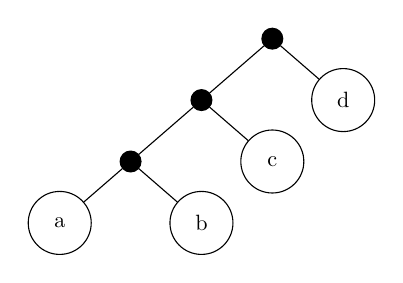
\begin{tikzpicture}[
  every node/.style={draw, circle, minimum size=1cm,scale=0.8},
  level distance=1.3cm,
  level 1/.style={sibling distance=3cm},
  level 2/.style={sibling distance=3cm},
  level 3/.style={sibling distance=3cm},
  scale=0.6
]
  \node[fill,circle,minimum size=.1cm] {}
    child {
      node[fill,circle,minimum size=.1cm] {}
      child{
        node[fill,circle,minimum size=.1cm] {}
        child {node {a}}
        child {node {b}}}
      child{ node {c}}}
    child {node {d}};
\end{tikzpicture}
}
&
{
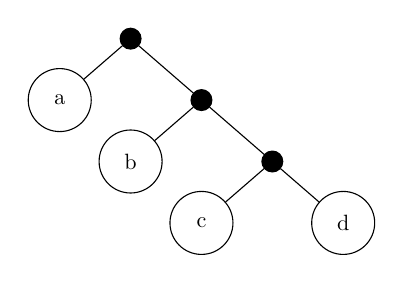
\begin{tikzpicture}[
  every node/.style={draw, circle, minimum size=1cm,scale=0.8},
  level distance=1.3cm,
  level 1/.style={sibling distance=3cm},
  level 2/.style={sibling distance=3cm},
  level 3/.style={sibling distance=3cm},
  scale=0.6
]
  \node[fill,circle,minimum size=.1cm] {}
    child[draw=none] {node {a}}
    child {node[fill,circle,minimum size=.1cm] {}
      child[draw=none] {node {b}}
      child {node[fill,circle,minimum size=.1cm] {}
        child[draw=none] {node {c}}
        child {node {d}}}};
\end{tikzpicture}
}
\end{tabular}
\end{center}
\medskip

A left-nested tree such as $(((a, b), c), d)$---the left diagram---yields a
bottom-up fold, whereas a right-nested tree such as $(a, (b, (c, d)))$---the
right diagram---induces a top-down fold.  Moreover, this
representation can express shapes that cannot be captured by simple lists, for
example $((a,b),(c,d))$.

To connect such trees with array elements, we view arrays as
containers~\citep{containers} whose shapes are binary trees: every shape
determines a set of positions, and an array assigns an element to every
position.  We achieve representation independence
of arrays and shapes by defining a minimalist \emph{array theory}.  In this case we fix
an interface to shapes, indices and arrays; we define some constraints,
but the actual implementation of these structures will be given
by concrete models.  We define our array theory as follows:
\begin{AgdaSuppressSpace}
\begin{mathpar}
\codeblock{\begin{code} %[hide]%
\>[0]\AgdaKeyword{record}\AgdaSpace{}%
\AgdaRecord{Array}\AgdaSpace{}%
\AgdaSymbol{:}\AgdaSpace{}%
\AgdaPrimitive{Set₁}\AgdaSpace{}%
\AgdaKeyword{where}\<%
\\
\>[0][@{}l@{\AgdaIndent{0}}]%
\>[2]\AgdaKeyword{field}\<%
\end{code}
\begin{mathpar}
\codeblock{\begin{code}%
\>[2][@{}l@{\AgdaIndent{1}}]%
\>[4]\AgdaField{S}%
\>[10]\AgdaSymbol{:}\AgdaSpace{}%
\AgdaPrimitive{Set}\<%
\\
%
\>[4]\AgdaField{P}%
\>[10]\AgdaSymbol{:}\AgdaSpace{}%
\AgdaField{S}\AgdaSpace{}%
\AgdaSymbol{→}\AgdaSpace{}%
\AgdaPrimitive{Set}\<%
\\
%
\\[\AgdaEmptyExtraSkip]%
%
\>[4]\AgdaField{ι}%
\>[10]\AgdaSymbol{:}\AgdaSpace{}%
\AgdaDatatype{ℕ}\AgdaSpace{}%
\AgdaSymbol{→}\AgdaSpace{}%
\AgdaField{S}\<%
\\
%
\>[4]\AgdaOperator{\AgdaField{\AgdaUnderscore{}⊗\AgdaUnderscore{}}}%
\>[10]\AgdaSymbol{:}\AgdaSpace{}%
\AgdaField{S}\AgdaSpace{}%
\AgdaSymbol{→}\AgdaSpace{}%
\AgdaField{S}\AgdaSpace{}%
\AgdaSymbol{→}\AgdaSpace{}%
\AgdaField{S}\<%
\end{code}}
\and
\codeblock{\begin{code}%
%
\>[4]\AgdaField{ι-↔}%
\>[10]\AgdaSymbol{:}\AgdaSpace{}%
\AgdaField{P}\AgdaSpace{}%
\AgdaSymbol{(}\AgdaField{ι}\AgdaSpace{}%
\AgdaGeneralizable{n}\AgdaSymbol{)}\AgdaSpace{}%
\AgdaOperator{\AgdaFunction{↔}}\AgdaSpace{}%
\AgdaDatatype{Fin}\AgdaSpace{}%
\AgdaGeneralizable{n}\<%
\\
%
\>[4]\AgdaField{⊗-↔}%
\>[10]\AgdaSymbol{:}\AgdaSpace{}%
\AgdaSymbol{∀}\AgdaSpace{}%
\AgdaSymbol{\{}\AgdaBound{s}\AgdaSpace{}%
\AgdaBound{p}\AgdaSymbol{\}}\AgdaSpace{}%
\AgdaSymbol{→}\AgdaSpace{}%
\AgdaField{P}\AgdaSpace{}%
\AgdaSymbol{(}\AgdaBound{s}\AgdaSpace{}%
\AgdaOperator{\AgdaField{⊗}}\AgdaSpace{}%
\AgdaBound{p}\AgdaSymbol{)}\AgdaSpace{}%
\AgdaOperator{\AgdaFunction{↔}}\AgdaSpace{}%
\AgdaSymbol{(}\AgdaField{P}\AgdaSpace{}%
\AgdaBound{s}\AgdaSpace{}%
\AgdaOperator{\AgdaFunction{×}}\AgdaSpace{}%
\AgdaField{P}\AgdaSpace{}%
\AgdaBound{p}\AgdaSymbol{)}\<%
\\
%
\\[\AgdaEmptyExtraSkip]%
%
\>[4]\AgdaField{Ar}%
\>[10]\AgdaSymbol{:}\AgdaSpace{}%
\AgdaField{S}\AgdaSpace{}%
\AgdaSymbol{→}\AgdaSpace{}%
\AgdaPrimitive{Set}\AgdaSpace{}%
\AgdaSymbol{→}\AgdaSpace{}%
\AgdaPrimitive{Set}\<%
\\
%
\>[4]\AgdaField{Ar-↔}%
\>[10]\AgdaSymbol{:}\AgdaSpace{}%
\AgdaSymbol{∀}\AgdaSpace{}%
\AgdaSymbol{\{}\AgdaBound{s}\AgdaSymbol{\}}\AgdaSpace{}%
\AgdaSymbol{→}\AgdaSpace{}%
\AgdaSymbol{(}\AgdaField{P}\AgdaSpace{}%
\AgdaBound{s}\AgdaSpace{}%
\AgdaSymbol{→}\AgdaSpace{}%
\AgdaGeneralizable{X}\AgdaSymbol{)}\AgdaSpace{}%
\AgdaOperator{\AgdaFunction{↔}}\AgdaSpace{}%
\AgdaField{Ar}\AgdaSpace{}%
\AgdaBound{s}\AgdaSpace{}%
\AgdaGeneralizable{X}\<%
\end{code}}
\end{mathpar}}
\end{mathpar}
\end{AgdaSuppressSpace}

The theory draws inspiration from container theory~\citep{10.1007/3-540-36576-1_2},
introducing restrictions on the kind of shapes that are allowed,
and generalising the notion of container interpretation.

The theory consists of shapes \AR{S} and positions (indices) \AR{P}
within such shapes.  We require two constructors
for \AR{S}: \AR{ι} which lifts a given
natural number into \AR{S} and 
\AR{\_⊗\_} which builds a shape out of left and right sub-shapes.

Positions \AR{P} of a given shape \AB{s} characterise
all the valid indices into arrays of that shape.
We require two properties of \AR{P}.  Firstly, \AR{ι-↔} 
requires indices of a singleton shape \AR{ι} \AB{n} to be
isomorphic (denoted by \AF{↔}) to
the natural numbers $[0 \dots n)$ which is denoted by the type \AD{Fin} $n$.
Secondly, \AR{⊗-↔} requires
indices of a product shape to be isomorphic to the product
of left and right sub-indices.

For readers familiar with
universes, our theory says that (\AR{S}, \AR{P}) is a
monoidal\footnote{
A universe $(U,\,El)$ with a monoid structure $(U, \epsilon, *)$ that $El$
maps to the monoid (\AF{Set}, \AD{⊤}, \AD{\_×\_}): $El\,\epsilon$ is
\AD{⊤} and $El\,(a * b)$ is $El\,a$ \AD{×} $El\,b$.  Technically, as in
monoidal categories, all of these laws hold up to isomorphism.
} universe where (\AR{ι} 1) is a unit.

\AR{Ar} is a type of arrays and \AR{Ar-↔} requires 
\AR{Ar} of shape \AB{s} to be isomorphic to a function
from indices of shape \AB{s} to array elements.
Note a distinction with the container theory, where
the interpretation of the container (\AB{S}, \AB{P}) for some \AB{X}
is fixed to \AF{Σ} (s : \AB{S}) (\AB{P} \AB{s} → \AB{X}).
Here we only say that \AR{Ar} \emph{has to be} a
representable functor~\citep{SB_1958-1960__5__369_0}
(\ie{} (\AR{Ar} \AB{s}) is isomorphic to (\AR{P} \AB{s} → \AB{X})).
The concrete storage layout is left to the model.

\subsection{\label{sec:arrop}Array operations}

For any array model $A$, we can expand the isomorphisms of
the array theory into operations on shapes, indices, and arrays.
We group these operations into a module that we call \AM{ArOps}
which is parametrised by $A$:
\begin{AgdaSuppressSpace}
\begin{code}%
\>[0]\AgdaKeyword{module}\AgdaSpace{}%
\AgdaModule{ArOps}\AgdaSpace{}%
\AgdaSymbol{(}\AgdaBound{A}\AgdaSpace{}%
\AgdaSymbol{:}\AgdaSpace{}%
\AgdaRecord{Array}\AgdaSymbol{)}\AgdaSpace{}%
\AgdaKeyword{where}\<%
\end{code}
\begin{code}[hide]%
\>[0][@{}l@{\AgdaIndent{1}}]%
\>[2]\AgdaKeyword{open}\AgdaSpace{}%
\AgdaModule{Array}\AgdaSpace{}%
\AgdaBound{A}\<%
\\
%
\>[2]\AgdaKeyword{private}\AgdaSpace{}%
\AgdaKeyword{variable}\<%
\\
\>[2][@{}l@{\AgdaIndent{0}}]%
\>[4]\AgdaGeneralizable{s}\AgdaSpace{}%
\AgdaGeneralizable{p}\AgdaSpace{}%
\AgdaGeneralizable{l}\AgdaSpace{}%
\AgdaGeneralizable{r}\AgdaSpace{}%
\AgdaSymbol{:}\AgdaSpace{}%
\AgdaField{S}\<%
\end{code}
\begin{mathpar}
\codeblock{\begin{code}%
%
\>[2]\AgdaFunction{imap}%
\>[8]\AgdaSymbol{:}\AgdaSpace{}%
\AgdaSymbol{(}\AgdaField{P}\AgdaSpace{}%
\AgdaGeneralizable{s}\AgdaSpace{}%
\AgdaSymbol{→}\AgdaSpace{}%
\AgdaGeneralizable{X}\AgdaSymbol{)}\AgdaSpace{}%
\AgdaSymbol{→}\AgdaSpace{}%
\AgdaField{Ar}\AgdaSpace{}%
\AgdaGeneralizable{s}\AgdaSpace{}%
\AgdaGeneralizable{X}\<%
\\
%
\>[2]\AgdaOperator{\AgdaFunction{\AgdaUnderscore{}[\AgdaUnderscore{}]}}%
\>[8]\AgdaSymbol{:}\AgdaSpace{}%
\AgdaField{Ar}\AgdaSpace{}%
\AgdaGeneralizable{s}\AgdaSpace{}%
\AgdaGeneralizable{X}\AgdaSpace{}%
\AgdaSymbol{→}\AgdaSpace{}%
\AgdaSymbol{(}\AgdaField{P}\AgdaSpace{}%
\AgdaGeneralizable{s}\AgdaSpace{}%
\AgdaSymbol{→}\AgdaSpace{}%
\AgdaGeneralizable{X}\AgdaSymbol{)}\<%
\\
\>[0]\<%
\end{code}}
\and
\codeblock{\begin{code}%
\>[0][@{}l@{\AgdaIndent{1}}]%
\>[2]\AgdaFunction{φ}%
\>[7]\AgdaSymbol{:}\AgdaSpace{}%
\AgdaDatatype{Fin}\AgdaSpace{}%
\AgdaGeneralizable{n}\AgdaSpace{}%
\AgdaSymbol{→}\AgdaSpace{}%
\AgdaField{P}\AgdaSpace{}%
\AgdaSymbol{(}\AgdaField{ι}\AgdaSpace{}%
\AgdaGeneralizable{n}\AgdaSymbol{)}\<%
\\
%
\>[2]\AgdaFunction{ψ}%
\>[7]\AgdaSymbol{:}\AgdaSpace{}%
\AgdaField{P}\AgdaSpace{}%
\AgdaSymbol{(}\AgdaField{ι}\AgdaSpace{}%
\AgdaGeneralizable{n}\AgdaSymbol{)}\AgdaSpace{}%
\AgdaSymbol{→}\AgdaSpace{}%
\AgdaDatatype{Fin}\AgdaSpace{}%
\AgdaGeneralizable{n}\<%
\\
\>[0]\<%
\end{code}}
\and
\codeblock{\begin{code}%
\>[0][@{}l@{\AgdaIndent{1}}]%
\>[2]\AgdaFunction{fst}%
\>[7]\AgdaSymbol{:}\AgdaSpace{}%
\AgdaField{P}\AgdaSpace{}%
\AgdaSymbol{(}\AgdaGeneralizable{l}\AgdaSpace{}%
\AgdaOperator{\AgdaField{⊗}}\AgdaSpace{}%
\AgdaGeneralizable{r}\AgdaSymbol{)}\AgdaSpace{}%
\AgdaSymbol{→}\AgdaSpace{}%
\AgdaField{P}\AgdaSpace{}%
\AgdaGeneralizable{l}\<%
\\
%
\>[2]\AgdaFunction{snd}%
\>[7]\AgdaSymbol{:}\AgdaSpace{}%
\AgdaField{P}\AgdaSpace{}%
\AgdaSymbol{(}\AgdaGeneralizable{l}\AgdaSpace{}%
\AgdaOperator{\AgdaField{⊗}}\AgdaSpace{}%
\AgdaGeneralizable{r}\AgdaSymbol{)}\AgdaSpace{}%
\AgdaSymbol{→}\AgdaSpace{}%
\AgdaField{P}\AgdaSpace{}%
\AgdaGeneralizable{r}\<%
\\
%
\>[2]\AgdaOperator{\AgdaFunction{\AgdaUnderscore{}⊛\AgdaUnderscore{}}}%
\>[7]\AgdaSymbol{:}\AgdaSpace{}%
\AgdaField{P}\AgdaSpace{}%
\AgdaGeneralizable{l}\AgdaSpace{}%
\AgdaSymbol{→}\AgdaSpace{}%
\AgdaField{P}\AgdaSpace{}%
\AgdaGeneralizable{r}\AgdaSpace{}%
\AgdaSymbol{→}\AgdaSpace{}%
\AgdaField{P}\AgdaSpace{}%
\AgdaSymbol{(}\AgdaGeneralizable{l}\AgdaSpace{}%
\AgdaOperator{\AgdaField{⊗}}\AgdaSpace{}%
\AgdaGeneralizable{r}\AgdaSymbol{)}\<%
\end{code}}
\end{mathpar}
\end{AgdaSuppressSpace}
The forward direction of the \AR{Ar-↔} isomorphism gives us
a function that we call \AF{imap} (sometimes called
\emph{tabulate}); the backward direction gives us selections into
arrays for which we use a C-like notation \AF{\_[\_]}.
Similarly, when expanding \AR{ι-↔} and \AR{⊗-↔}
we obtain convenient operations on indices: \AF{φ} and \AF{ψ}
which translate between the one-dimensional indices and \AD{Fin} $n$;
\AF{fst} and \AF{snd} project left and right sub-indices from
the index of a product shape; and \AF{\_⊛\_} makes an index
of a product shape from two sub-indices of the corresponding
sub-shapes.
\begin{code}[hide]%
%
\>[2]\AgdaBound{i}\AgdaSpace{}%
\AgdaOperator{\AgdaFunction{⊛}}\AgdaSpace{}%
\AgdaBound{j}\AgdaSpace{}%
\AgdaSymbol{=}\AgdaSpace{}%
\AgdaField{Inverse.from}\AgdaSpace{}%
\AgdaField{⊗-↔}\AgdaSpace{}%
\AgdaSymbol{(}\AgdaBound{i}\AgdaSpace{}%
\AgdaOperator{\AgdaInductiveConstructor{,}}\AgdaSpace{}%
\AgdaBound{j}\AgdaSymbol{)}\<%
\\
%
\>[2]\AgdaFunction{φ}%
\>[8]\AgdaSymbol{=}\AgdaSpace{}%
\AgdaField{Inverse.from}\AgdaSpace{}%
\AgdaField{ι-↔}\<%
\\
%
\>[2]\AgdaFunction{ψ}%
\>[8]\AgdaSymbol{=}\AgdaSpace{}%
\AgdaField{Inverse.to}\AgdaSpace{}%
\AgdaField{ι-↔}\<%
\\
%
\>[2]\AgdaFunction{snd}%
\>[8]\AgdaSymbol{=}\AgdaSpace{}%
\AgdaField{proj₂}\AgdaSpace{}%
\AgdaOperator{\AgdaFunction{∘}}\AgdaSpace{}%
\AgdaField{Inverse.to}\AgdaSpace{}%
\AgdaField{⊗-↔}\<%
\\
%
\>[2]\AgdaFunction{fst}%
\>[8]\AgdaSymbol{=}\AgdaSpace{}%
\AgdaField{proj₁}\AgdaSpace{}%
\AgdaOperator{\AgdaFunction{∘}}\AgdaSpace{}%
\AgdaField{Inverse.to}\AgdaSpace{}%
\AgdaField{⊗-↔}\<%
\\
%
\>[2]\AgdaFunction{imap}%
\>[8]\AgdaSymbol{=}\AgdaSpace{}%
\AgdaField{Inverse.to}\AgdaSpace{}%
\AgdaField{Ar-↔}\<%
\\
%
\>[2]\AgdaOperator{\AgdaFunction{\AgdaUnderscore{}[\AgdaUnderscore{}]}}%
\>[8]\AgdaSymbol{=}\AgdaSpace{}%
\AgdaField{Inverse.from}\AgdaSpace{}%
\AgdaField{Ar-↔}\<%
\\
%
\\[\AgdaEmptyExtraSkip]%
%
\>[2]\AgdaKeyword{private}\AgdaSpace{}%
\AgdaKeyword{variable}\<%
\\
\>[2][@{}l@{\AgdaIndent{0}}]%
\>[4]\AgdaGeneralizable{a}\AgdaSpace{}%
\AgdaGeneralizable{b}\AgdaSpace{}%
\AgdaGeneralizable{c}\AgdaSpace{}%
\AgdaSymbol{:}\AgdaSpace{}%
\AgdaField{Ar}\AgdaSpace{}%
\AgdaGeneralizable{s}\AgdaSpace{}%
\AgdaGeneralizable{X}\<%
\end{code}


\subsubsection{Equality of arrays}
Using selection, we can define the notion of point-wise
equality of two arrays \AF{\_≈ₐ\_} and show that \AF{≈ₐ} is an 
equivalence relation, meaning that \AF{Ar} with \AF{≈ₐ} is a setoid.
Throughout the paper we use the term setoid in its type-theoretic sense: a type
equipped with an equivalence relation, which need not be proof-irrelevant.
\begin{mathpar}
\codeblock{\begin{code}%
%
\>[2]\AgdaOperator{\AgdaFunction{\AgdaUnderscore{}≈ₐ\AgdaUnderscore{}}}\AgdaSpace{}%
\AgdaSymbol{:}\AgdaSpace{}%
\AgdaField{Ar}\AgdaSpace{}%
\AgdaGeneralizable{s}\AgdaSpace{}%
\AgdaGeneralizable{X}\AgdaSpace{}%
\AgdaSymbol{→}\AgdaSpace{}%
\AgdaField{Ar}\AgdaSpace{}%
\AgdaGeneralizable{s}\AgdaSpace{}%
\AgdaGeneralizable{X}\AgdaSpace{}%
\AgdaSymbol{→}\AgdaSpace{}%
\AgdaPrimitive{Set}\<%
\\
%
\>[2]\AgdaBound{a}\AgdaSpace{}%
\AgdaOperator{\AgdaFunction{≈ₐ}}\AgdaSpace{}%
\AgdaBound{b}\AgdaSpace{}%
\AgdaSymbol{=}\AgdaSpace{}%
\AgdaSymbol{∀}\AgdaSpace{}%
\AgdaBound{ix}\AgdaSpace{}%
\AgdaSymbol{→}\AgdaSpace{}%
\AgdaBound{a}\AgdaSpace{}%
\AgdaOperator{\AgdaFunction{[}}\AgdaSpace{}%
\AgdaBound{ix}\AgdaSpace{}%
\AgdaOperator{\AgdaFunction{]}}\AgdaSpace{}%
\AgdaOperator{\AgdaDatatype{≡}}\AgdaSpace{}%
\AgdaBound{b}\AgdaSpace{}%
\AgdaOperator{\AgdaFunction{[}}\AgdaSpace{}%
\AgdaBound{ix}\AgdaSpace{}%
\AgdaOperator{\AgdaFunction{]}}\<%
\end{code}}
\and
\codeblock{\begin{code}%
%
\>[2]\AgdaFunction{refl-≈ₐ}%
\>[12]\AgdaSymbol{:}\AgdaSpace{}%
\AgdaGeneralizable{a}\AgdaSpace{}%
\AgdaOperator{\AgdaFunction{≈ₐ}}\AgdaSpace{}%
\AgdaGeneralizable{a}\<%
\\
%
\>[2]\AgdaFunction{sym-≈ₐ}%
\>[12]\AgdaSymbol{:}\AgdaSpace{}%
\AgdaGeneralizable{a}\AgdaSpace{}%
\AgdaOperator{\AgdaFunction{≈ₐ}}\AgdaSpace{}%
\AgdaGeneralizable{b}\AgdaSpace{}%
\AgdaSymbol{→}\AgdaSpace{}%
\AgdaGeneralizable{b}\AgdaSpace{}%
\AgdaOperator{\AgdaFunction{≈ₐ}}\AgdaSpace{}%
\AgdaGeneralizable{a}\<%
\\
%
\>[2]\AgdaFunction{trans-≈ₐ}%
\>[12]\AgdaSymbol{:}\AgdaSpace{}%
\AgdaGeneralizable{a}\AgdaSpace{}%
\AgdaOperator{\AgdaFunction{≈ₐ}}\AgdaSpace{}%
\AgdaGeneralizable{b}\AgdaSpace{}%
\AgdaSymbol{→}\AgdaSpace{}%
\AgdaGeneralizable{b}\AgdaSpace{}%
\AgdaOperator{\AgdaFunction{≈ₐ}}\AgdaSpace{}%
\AgdaGeneralizable{c}\AgdaSpace{}%
\AgdaSymbol{→}\AgdaSpace{}%
\AgdaGeneralizable{a}\AgdaSpace{}%
\AgdaOperator{\AgdaFunction{≈ₐ}}\AgdaSpace{}%
\AgdaGeneralizable{c}\<%
\end{code}}
\end{mathpar}
\begin{code}[hide]%
%
\>[2]\AgdaFunction{refl-≈ₐ}\AgdaSpace{}%
\AgdaBound{ix}\AgdaSpace{}%
\AgdaSymbol{=}\AgdaSpace{}%
\AgdaInductiveConstructor{refl}\<%
\\
%
\>[2]\AgdaFunction{sym-≈ₐ}\AgdaSpace{}%
\AgdaBound{a≈b}\AgdaSpace{}%
\AgdaBound{ix}\AgdaSpace{}%
\AgdaSymbol{=}\AgdaSpace{}%
\AgdaFunction{sym}\AgdaSpace{}%
\AgdaSymbol{(}\AgdaBound{a≈b}\AgdaSpace{}%
\AgdaBound{ix}\AgdaSymbol{)}\<%
\\
%
\>[2]\AgdaFunction{trans-≈ₐ}\AgdaSpace{}%
\AgdaBound{a≈b}\AgdaSpace{}%
\AgdaBound{b≈c}\AgdaSpace{}%
\AgdaBound{ix}\AgdaSpace{}%
\AgdaSymbol{=}\AgdaSpace{}%
\AgdaFunction{trans}\AgdaSpace{}%
\AgdaSymbol{(}\AgdaBound{a≈b}\AgdaSpace{}%
\AgdaBound{ix}\AgdaSymbol{)}\AgdaSpace{}%
\AgdaSymbol{(}\AgdaBound{b≈c}\AgdaSpace{}%
\AgdaBound{ix}\AgdaSymbol{)}\<%
\\
\>[0]\<%
\\
%
\\[\AgdaEmptyExtraSkip]%
%
\>[2]\AgdaKeyword{import}\AgdaSpace{}%
\AgdaModule{Relation.Binary.Reasoning.Setoid}\AgdaSpace{}%
\AgdaSymbol{as}\AgdaSpace{}%
\AgdaModule{EqReasoning}\<%
\\
%
\\[\AgdaEmptyExtraSkip]%
%
\>[2]\AgdaFunction{≈ₐ-isEquiv}\AgdaSpace{}%
\AgdaSymbol{:}\AgdaSpace{}%
\AgdaSymbol{∀}\AgdaSpace{}%
\AgdaSymbol{\{}\AgdaBound{s}\AgdaSpace{}%
\AgdaBound{X}\AgdaSymbol{\}}\AgdaSpace{}%
\AgdaSymbol{→}\AgdaSpace{}%
\AgdaRecord{IsEquivalence}\AgdaSpace{}%
\AgdaSymbol{(}\AgdaOperator{\AgdaFunction{\AgdaUnderscore{}≈ₐ\AgdaUnderscore{}}}\AgdaSpace{}%
\AgdaSymbol{\{}\AgdaBound{s}\AgdaSymbol{\}}\AgdaSpace{}%
\AgdaSymbol{\{}\AgdaBound{X}\AgdaSymbol{\})}\<%
\\
%
\>[2]\AgdaFunction{≈ₐ-isEquiv}\AgdaSpace{}%
\AgdaSymbol{=}\AgdaSpace{}%
\AgdaKeyword{record}\AgdaSpace{}%
\AgdaSymbol{\{}\AgdaSpace{}%
\AgdaField{refl}\AgdaSpace{}%
\AgdaSymbol{=}\AgdaSpace{}%
\AgdaFunction{refl-≈ₐ}\AgdaSpace{}%
\AgdaSymbol{;}\AgdaSpace{}%
\AgdaField{sym}\AgdaSpace{}%
\AgdaSymbol{=}\AgdaSpace{}%
\AgdaFunction{sym-≈ₐ}\AgdaSpace{}%
\AgdaSymbol{;}\AgdaSpace{}%
\AgdaField{trans}\AgdaSpace{}%
\AgdaSymbol{=}\AgdaSpace{}%
\AgdaFunction{trans-≈ₐ}\AgdaSymbol{\}}\<%
\\
%
\\[\AgdaEmptyExtraSkip]%
%
\>[2]\AgdaFunction{ArSetoid}\AgdaSpace{}%
\AgdaSymbol{:}\AgdaSpace{}%
\AgdaSymbol{∀}\AgdaSpace{}%
\AgdaSymbol{\{}\AgdaBound{s}\AgdaSpace{}%
\AgdaBound{X}\AgdaSymbol{\}}\AgdaSpace{}%
\AgdaSymbol{→}\AgdaSpace{}%
\AgdaRecord{Setoid}\AgdaSpace{}%
\AgdaSymbol{\AgdaUnderscore{}}\AgdaSpace{}%
\AgdaSymbol{\AgdaUnderscore{}}\<%
\\
%
\>[2]\AgdaFunction{ArSetoid}\AgdaSpace{}%
\AgdaSymbol{\{}\AgdaBound{s}\AgdaSymbol{\}}\AgdaSpace{}%
\AgdaSymbol{\{}\AgdaBound{X}\AgdaSymbol{\}}\AgdaSpace{}%
\AgdaSymbol{=}\AgdaSpace{}%
\AgdaKeyword{record}\AgdaSpace{}%
\AgdaSymbol{\{}\AgdaSpace{}%
\AgdaField{isEquivalence}\AgdaSpace{}%
\AgdaSymbol{=}\AgdaSpace{}%
\AgdaFunction{≈ₐ-isEquiv}\AgdaSpace{}%
\AgdaSymbol{\{}\AgdaBound{s}\AgdaSymbol{\}}\AgdaSpace{}%
\AgdaSymbol{\{}\AgdaBound{X}\AgdaSymbol{\}\}}\<%
\\
%
\\[\AgdaEmptyExtraSkip]%
%
\>[2]\AgdaKeyword{module}\AgdaSpace{}%
\AgdaModule{ArReasoning}\AgdaSpace{}%
\AgdaSymbol{\{}\AgdaBound{s}\AgdaSymbol{\}}\AgdaSpace{}%
\AgdaSymbol{\{}\AgdaBound{X}\AgdaSymbol{\}}\AgdaSpace{}%
\AgdaSymbol{=}\AgdaSpace{}%
\AgdaModule{EqReasoning}\AgdaSpace{}%
\AgdaSymbol{(}\AgdaFunction{ArSetoid}\AgdaSpace{}%
\AgdaSymbol{\{}\AgdaBound{s}\AgdaSymbol{\}}\AgdaSpace{}%
\AgdaSymbol{\{}\AgdaBound{X}\AgdaSymbol{\})}\<%
\end{code}

\begin{code}[hide]%
%
\>[2]\AgdaComment{--\ Named\ consequences\ of\ the\ isomorphisms\ of\ the\ array\ theory.}\<%
\\
%
\>[2]\AgdaFunction{sel∘imap}\AgdaSpace{}%
\AgdaSymbol{:}\AgdaSpace{}%
\AgdaSymbol{∀}\AgdaSpace{}%
\AgdaSymbol{\{}\AgdaBound{s}\AgdaSpace{}%
\AgdaBound{X}\AgdaSymbol{\}}\AgdaSpace{}%
\AgdaSymbol{(}\AgdaBound{a}\AgdaSpace{}%
\AgdaSymbol{:}\AgdaSpace{}%
\AgdaField{P}\AgdaSpace{}%
\AgdaBound{s}\AgdaSpace{}%
\AgdaSymbol{→}\AgdaSpace{}%
\AgdaBound{X}\AgdaSymbol{)}\AgdaSpace{}%
\AgdaSymbol{→}\AgdaSpace{}%
\AgdaFunction{imap}\AgdaSpace{}%
\AgdaBound{a}\AgdaSpace{}%
\AgdaOperator{\AgdaFunction{[\AgdaUnderscore{}]}}\AgdaSpace{}%
\AgdaOperator{\AgdaDatatype{≡}}\AgdaSpace{}%
\AgdaBound{a}\<%
\\
%
\>[2]\AgdaFunction{sel∘imap}\AgdaSpace{}%
\AgdaSymbol{=}\AgdaSpace{}%
\AgdaFunction{Inverse.strictlyInverseʳ}\AgdaSpace{}%
\AgdaField{Ar-↔}\<%
\\
%
\\[\AgdaEmptyExtraSkip]%
%
\>[2]\AgdaFunction{sel-imap}\AgdaSpace{}%
\AgdaSymbol{:}\AgdaSpace{}%
\AgdaSymbol{∀}\AgdaSpace{}%
\AgdaSymbol{\{}\AgdaBound{s}\AgdaSpace{}%
\AgdaBound{X}\AgdaSymbol{\}}\AgdaSpace{}%
\AgdaSymbol{(}\AgdaBound{a}\AgdaSpace{}%
\AgdaSymbol{:}\AgdaSpace{}%
\AgdaField{P}\AgdaSpace{}%
\AgdaBound{s}\AgdaSpace{}%
\AgdaSymbol{→}\AgdaSpace{}%
\AgdaBound{X}\AgdaSymbol{)}\AgdaSpace{}%
\AgdaSymbol{(}\AgdaBound{i}\AgdaSpace{}%
\AgdaSymbol{:}\AgdaSpace{}%
\AgdaField{P}\AgdaSpace{}%
\AgdaBound{s}\AgdaSymbol{)}\AgdaSpace{}%
\AgdaSymbol{→}\AgdaSpace{}%
\AgdaFunction{imap}\AgdaSpace{}%
\AgdaBound{a}\AgdaSpace{}%
\AgdaOperator{\AgdaFunction{[}}\AgdaSpace{}%
\AgdaBound{i}\AgdaSpace{}%
\AgdaOperator{\AgdaFunction{]}}\AgdaSpace{}%
\AgdaOperator{\AgdaDatatype{≡}}\AgdaSpace{}%
\AgdaBound{a}\AgdaSpace{}%
\AgdaBound{i}\<%
\\
%
\>[2]\AgdaFunction{sel-imap}\AgdaSpace{}%
\AgdaBound{a}\AgdaSpace{}%
\AgdaBound{i}\AgdaSpace{}%
\AgdaSymbol{=}\AgdaSpace{}%
\AgdaFunction{cong}\AgdaSpace{}%
\AgdaSymbol{(}\AgdaOperator{\AgdaFunction{\AgdaUnderscore{}\$}}\AgdaSpace{}%
\AgdaBound{i}\AgdaSymbol{)}\AgdaSpace{}%
\AgdaSymbol{(}\AgdaFunction{sel∘imap}\AgdaSpace{}%
\AgdaBound{a}\AgdaSymbol{)}\<%
\\
%
\\[\AgdaEmptyExtraSkip]%
%
\>[2]\AgdaFunction{ψ-φ}\AgdaSpace{}%
\AgdaSymbol{:}\AgdaSpace{}%
\AgdaSymbol{(}\AgdaBound{i}\AgdaSpace{}%
\AgdaSymbol{:}\AgdaSpace{}%
\AgdaDatatype{Fin}\AgdaSpace{}%
\AgdaGeneralizable{n}\AgdaSymbol{)}\AgdaSpace{}%
\AgdaSymbol{→}\AgdaSpace{}%
\AgdaFunction{ψ}\AgdaSpace{}%
\AgdaSymbol{(}\AgdaFunction{φ}\AgdaSpace{}%
\AgdaBound{i}\AgdaSymbol{)}\AgdaSpace{}%
\AgdaOperator{\AgdaDatatype{≡}}\AgdaSpace{}%
\AgdaBound{i}\<%
\\
%
\>[2]\AgdaFunction{ψ-φ}\AgdaSpace{}%
\AgdaSymbol{=}\AgdaSpace{}%
\AgdaFunction{Inverse.strictlyInverseˡ}\AgdaSpace{}%
\AgdaField{ι-↔}\<%
\\
%
\\[\AgdaEmptyExtraSkip]%
%
\>[2]\AgdaFunction{φ-ψ}\AgdaSpace{}%
\AgdaSymbol{:}\AgdaSpace{}%
\AgdaSymbol{(}\AgdaBound{i}\AgdaSpace{}%
\AgdaSymbol{:}\AgdaSpace{}%
\AgdaField{P}\AgdaSpace{}%
\AgdaSymbol{(}\AgdaField{ι}\AgdaSpace{}%
\AgdaGeneralizable{n}\AgdaSymbol{))}\AgdaSpace{}%
\AgdaSymbol{→}\AgdaSpace{}%
\AgdaFunction{φ}\AgdaSpace{}%
\AgdaSymbol{(}\AgdaFunction{ψ}\AgdaSpace{}%
\AgdaBound{i}\AgdaSymbol{)}\AgdaSpace{}%
\AgdaOperator{\AgdaDatatype{≡}}\AgdaSpace{}%
\AgdaBound{i}\<%
\\
%
\>[2]\AgdaFunction{φ-ψ}\AgdaSpace{}%
\AgdaSymbol{=}\AgdaSpace{}%
\AgdaFunction{Inverse.strictlyInverseʳ}\AgdaSpace{}%
\AgdaField{ι-↔}\<%
\\
%
\\[\AgdaEmptyExtraSkip]%
%
\>[2]\AgdaFunction{fst-snd-⊛}\AgdaSpace{}%
\AgdaSymbol{:}\AgdaSpace{}%
\AgdaSymbol{(}\AgdaBound{i}\AgdaSpace{}%
\AgdaSymbol{:}\AgdaSpace{}%
\AgdaField{P}\AgdaSpace{}%
\AgdaGeneralizable{l}\AgdaSymbol{)}\AgdaSpace{}%
\AgdaSymbol{(}\AgdaBound{j}\AgdaSpace{}%
\AgdaSymbol{:}\AgdaSpace{}%
\AgdaField{P}\AgdaSpace{}%
\AgdaGeneralizable{r}\AgdaSymbol{)}\AgdaSpace{}%
\AgdaSymbol{→}\AgdaSpace{}%
\AgdaField{Inverse.to}\AgdaSpace{}%
\AgdaField{⊗-↔}\AgdaSpace{}%
\AgdaSymbol{(}\AgdaBound{i}\AgdaSpace{}%
\AgdaOperator{\AgdaFunction{⊛}}\AgdaSpace{}%
\AgdaBound{j}\AgdaSymbol{)}\AgdaSpace{}%
\AgdaOperator{\AgdaDatatype{≡}}\AgdaSpace{}%
\AgdaSymbol{(}\AgdaBound{i}\AgdaSpace{}%
\AgdaOperator{\AgdaInductiveConstructor{,}}\AgdaSpace{}%
\AgdaBound{j}\AgdaSymbol{)}\<%
\\
%
\>[2]\AgdaFunction{fst-snd-⊛}\AgdaSpace{}%
\AgdaBound{i}\AgdaSpace{}%
\AgdaBound{j}\AgdaSpace{}%
\AgdaSymbol{=}\AgdaSpace{}%
\AgdaFunction{Inverse.strictlyInverseˡ}\AgdaSpace{}%
\AgdaField{⊗-↔}\AgdaSpace{}%
\AgdaSymbol{(}\AgdaBound{i}\AgdaSpace{}%
\AgdaOperator{\AgdaInductiveConstructor{,}}\AgdaSpace{}%
\AgdaBound{j}\AgdaSymbol{)}\<%
\\
%
\\[\AgdaEmptyExtraSkip]%
%
\>[2]\AgdaFunction{fst-⊛}\AgdaSpace{}%
\AgdaSymbol{:}\AgdaSpace{}%
\AgdaSymbol{(}\AgdaBound{i}\AgdaSpace{}%
\AgdaSymbol{:}\AgdaSpace{}%
\AgdaField{P}\AgdaSpace{}%
\AgdaGeneralizable{l}\AgdaSymbol{)}\AgdaSpace{}%
\AgdaSymbol{(}\AgdaBound{j}\AgdaSpace{}%
\AgdaSymbol{:}\AgdaSpace{}%
\AgdaField{P}\AgdaSpace{}%
\AgdaGeneralizable{r}\AgdaSymbol{)}\AgdaSpace{}%
\AgdaSymbol{→}\AgdaSpace{}%
\AgdaFunction{fst}\AgdaSpace{}%
\AgdaSymbol{(}\AgdaBound{i}\AgdaSpace{}%
\AgdaOperator{\AgdaFunction{⊛}}\AgdaSpace{}%
\AgdaBound{j}\AgdaSymbol{)}\AgdaSpace{}%
\AgdaOperator{\AgdaDatatype{≡}}\AgdaSpace{}%
\AgdaBound{i}\<%
\\
%
\>[2]\AgdaFunction{fst-⊛}\AgdaSpace{}%
\AgdaBound{i}\AgdaSpace{}%
\AgdaBound{j}\AgdaSpace{}%
\AgdaSymbol{=}\AgdaSpace{}%
\AgdaFunction{cong}\AgdaSpace{}%
\AgdaField{proj₁}\AgdaSpace{}%
\AgdaSymbol{(}\AgdaFunction{fst-snd-⊛}\AgdaSpace{}%
\AgdaBound{i}\AgdaSpace{}%
\AgdaBound{j}\AgdaSymbol{)}\<%
\\
%
\\[\AgdaEmptyExtraSkip]%
%
\>[2]\AgdaFunction{snd-⊛}\AgdaSpace{}%
\AgdaSymbol{:}\AgdaSpace{}%
\AgdaSymbol{(}\AgdaBound{i}\AgdaSpace{}%
\AgdaSymbol{:}\AgdaSpace{}%
\AgdaField{P}\AgdaSpace{}%
\AgdaGeneralizable{l}\AgdaSymbol{)}\AgdaSpace{}%
\AgdaSymbol{(}\AgdaBound{j}\AgdaSpace{}%
\AgdaSymbol{:}\AgdaSpace{}%
\AgdaField{P}\AgdaSpace{}%
\AgdaGeneralizable{r}\AgdaSymbol{)}\AgdaSpace{}%
\AgdaSymbol{→}\AgdaSpace{}%
\AgdaFunction{snd}\AgdaSpace{}%
\AgdaSymbol{(}\AgdaBound{i}\AgdaSpace{}%
\AgdaOperator{\AgdaFunction{⊛}}\AgdaSpace{}%
\AgdaBound{j}\AgdaSymbol{)}\AgdaSpace{}%
\AgdaOperator{\AgdaDatatype{≡}}\AgdaSpace{}%
\AgdaBound{j}\<%
\\
%
\>[2]\AgdaFunction{snd-⊛}\AgdaSpace{}%
\AgdaBound{i}\AgdaSpace{}%
\AgdaBound{j}\AgdaSpace{}%
\AgdaSymbol{=}\AgdaSpace{}%
\AgdaFunction{cong}\AgdaSpace{}%
\AgdaField{proj₂}\AgdaSpace{}%
\AgdaSymbol{(}\AgdaFunction{fst-snd-⊛}\AgdaSpace{}%
\AgdaBound{i}\AgdaSpace{}%
\AgdaBound{j}\AgdaSymbol{)}\<%
\\
%
\\[\AgdaEmptyExtraSkip]%
%
\>[2]\AgdaFunction{⊛-η}\AgdaSpace{}%
\AgdaSymbol{:}\AgdaSpace{}%
\AgdaSymbol{(}\AgdaBound{i}\AgdaSpace{}%
\AgdaSymbol{:}\AgdaSpace{}%
\AgdaField{P}\AgdaSpace{}%
\AgdaSymbol{(}\AgdaGeneralizable{l}\AgdaSpace{}%
\AgdaOperator{\AgdaField{⊗}}\AgdaSpace{}%
\AgdaGeneralizable{r}\AgdaSymbol{))}\AgdaSpace{}%
\AgdaSymbol{→}\AgdaSpace{}%
\AgdaFunction{fst}\AgdaSpace{}%
\AgdaBound{i}\AgdaSpace{}%
\AgdaOperator{\AgdaFunction{⊛}}\AgdaSpace{}%
\AgdaFunction{snd}\AgdaSpace{}%
\AgdaBound{i}\AgdaSpace{}%
\AgdaOperator{\AgdaDatatype{≡}}\AgdaSpace{}%
\AgdaBound{i}\<%
\\
%
\>[2]\AgdaFunction{⊛-η}\AgdaSpace{}%
\AgdaSymbol{=}\AgdaSpace{}%
\AgdaFunction{Inverse.strictlyInverseʳ}\AgdaSpace{}%
\AgdaField{⊗-↔}\<%
\end{code}
